% 2007 年四川卷文科第 4 题：题图。
% 来源 PDF：普通高考/2007/2007四川文.pdf，SHA256 1318df44733ec939e8789379d6fa2115a2c6a63e84b73c1f2bf3c080007ce68c
% 原页：第 1 页（A3 三栏）第 1 栏，印刷页 411，图在题干下方。
% 重绘依据：斜投影正方体，A 左下、B 右下、A1 左上、B1 右上，D1 在 A1 右上方；可见棱实线、被遮棱与辅助线虚线；与文科原页逐线比对一致。
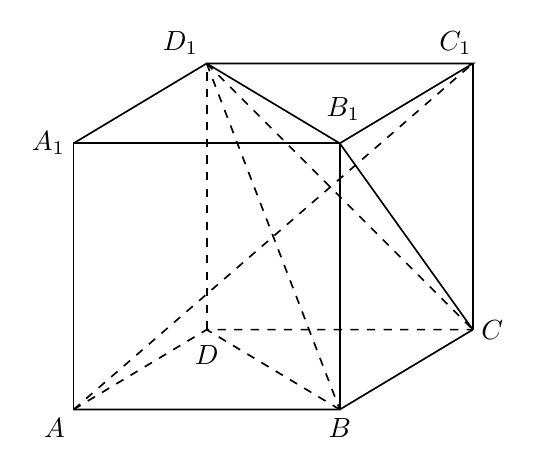
\begin{tikzpicture}[scale=1.3, semithick,
  every node/.style={inner sep=1.5pt}]
  \coordinate (A)  at (0,0);
  \coordinate (B)  at (2.6,0);
  \coordinate (A1) at (0,2.6);
  \coordinate (B1) at (2.6,2.6);
  \coordinate (D)  at (1.3,0.78);
  \coordinate (C)  at (3.9,0.78);
  \coordinate (D1) at (1.3,3.38);
  \coordinate (C1) at (3.9,3.38);
  % 不可见棱与不可见辅助线
  \draw[dashed] (A) -- (D) -- (C);
  \draw[dashed] (D) -- (D1);
  \draw[dashed] (B) -- (D);
  \draw[dashed] (D1) -- (B);
  \draw[dashed] (D1) -- (C);
  \draw[dashed] (A) -- (C1);
  % 可见棱
  \draw (A) -- (B) -- (C);
  \draw (A) -- (A1) -- (B1) -- (B);
  \draw (A1) -- (D1) -- (C1) -- (B1);
  \draw (C) -- (C1);
  % 可见辅助线
  \draw (B1) -- (D1);
  \draw (B1) -- (C);
  \node[anchor=north east] at ([xshift=-1pt,yshift=-1pt]A) {$A$};
  \node[anchor=north] at ([yshift=-1pt]B) {$B$};
  \node[anchor=west] at ([xshift=1pt]C) {$C$};
  \node[anchor=north] at ([yshift=-3pt]D) {$D$};
  \node[anchor=east] at ([xshift=-1pt]A1) {$A_1$};
  \node[anchor=south] at ([xshift=1pt,yshift=5pt]B1) {$B_1$};
  \node[anchor=south east] at ([xshift=1pt,yshift=1pt]C1) {$C_1$};
  \node[anchor=south east] at ([xshift=-1pt,yshift=1pt]D1) {$D_1$};
\end{tikzpicture}
